\documentclass[10pt]{article}
\usepackage{../../local}
\urlstyle{same}

\newcommand{\classcode}{EE 120}
\newcommand{\classname}{Signals and Systems}
\renewcommand{\maketitle}{%
\hrule height4pt
\large{Yutong Du \hfill \classcode}
\newline
\large{HW 01} \Large{\hfill \classname \hfill} \large{\today}
\hrule height4pt \vskip .7em
\small{Header styling inspired by CS 70: \url{https://www.eecs70.org/}}
\normalsize
}
\linespread{1.1}
\begin{document}
	\maketitle
	\section*{Collaborators}
	I worked with the following people:
	\begin{itemize}
		\item Teja Nivarthi: 3036508567
		\item Nikhil Maserang: 3036978230
	\end{itemize}
	I did this homework in \LaTeX{}, please let me know if there are any formatting preferences that would make 
	grading nicer. 
	\pagebreak

	\section*{Problem 1}
	Euler's formula is
	\[
	e^{i\theta} = \cos \theta + i \sin \theta
	\] 
	\begin{enumerate}[label=\alph*)]
		\item Derive the following identities using Euler's formula:
			\begin{enumerate}[label=\roman*)]
				\item \( \cos \theta = \frac{e^{i\theta} + e^{-i \theta}}{2} \)

					\begin{solution}
						The first thing to figure out is what \( e^{-i \theta} \) equals:
						\[
						e^{-i \theta} = \cos(-\theta) + i \sin (-\theta)
						\] 
						Since cosine is even, then \( \cos(-\theta) = \cos(\theta) \), and since sine is odd, 
						then \( \sin(-\theta) = -\sin(\theta) \). Therefore:
						\[
						e^{-i \theta} = \cos(\theta) - i \sin \theta
						\] 
						Therefore, we simplify the right hand side:
						\begin{align*}
							\frac{e^{i \theta} + e^{-i \theta}}{2} &= \frac{(\cos \theta + i \sin \theta) + 
							(\cos \theta - i \sin \theta)}{2} \\
							&= \frac{2\cos \theta}{2} \\
							&= \cos \theta 
						\end{align*}
						as desired. 
					\end{solution}
				\item \( \sin \theta = \frac{e^{i \theta} - e^{-i \theta}}{2i} \)
					\begin{solution}
						Similar to the previous problem, simplify the right hand side:
						\begin{align*}
							\frac{e^{i \theta} - e^{- i \theta}}{2i} &= \frac{(\cos \theta + i \sin \theta) - 
							(\cos \theta - i \sin \theta)}{2i} \\
							&= \frac{2i \sin \theta}{2i} \\
							&= \sin \theta 
						\end{align*}
						as desired. 
					\end{solution}
			\end{enumerate}
		\item Derive \textbf{de Moivre's Theorem:} for any real integer \( n \), 
			\[
				(\cos \theta + i \sin \theta)^{n} = \cos(n \theta) + i \sin (n \theta)
			\] 
			\begin{solution}
				We use Euler's formula on the left hand side: 
				\[
					(\cos \theta + i \sin \theta)^{n} = (e^{i \theta})^{n} = e^{i (n \theta)} = \cos(n \theta) + i 
					\sin (n \theta)
				\] 
			\end{solution}
		\item Show that any linear combination of a set sinusoids of frequency \( \omega \), is always a sinusoid
			of the same frequency, \textit{even if} each sinusoid has a distinct phase. In particular, show
			that 
			\[
			\sum_{k = 1}^{N}A_k \cos(\omega t + \phi_k) = A \cos (\omega t + \phi)
			\] 
			holds for some \( A  \) and \( \phi \), and derive expressions for \( A \) and \( \phi \) in terms of 
			\( A_k \) and \( \phi_k \). 

			\underline{Hint:} Recognize that any complex number can be written as \( Ae^{i \phi} \) for suitable 
			\( A \) and \( \phi \). Further notice that \( \sum_{k = 1}^{N}A_k e^{i \phi_k} \) is a complex 
			number. 

			\begin{solution}
				Here, we can express this sum in a slightly different way:
				\[
					\sum_{k = 1}^{N}A_k \cos(\omega t + \phi_k) =  \sum_{k = 1}^{N}\Re\left[A_k e^{i \omega t + \phi_k} \right]
				\] 
				Now, because the real part adds linearly, we can rewrite this as:
				\[
				\sum_{k = 1}^{N}\Re\left[ A_k e^{i \omega t + \phi_k} \right]  = \Re\left[ \sum_{k = 1}^{N}
				A_k e^{i \omega t + \phi_k}\right]  = \Re\left[ e^{i \omega t} \sum_{k = 1}^{N}A_k e^{\phi_k} \right] 
				\] 
				Now, since the sum of  \( A_k e^{i \phi_k} \) is some general complex number, we can write it as some 
				\( A e^{i \phi} \). Therefore:
				\[
				\Re\left[ e^{i \omega t}\sum_{k = 1}^{N}A_k e^{i \phi_k} \right]  = \Re\left[ e^{i \omega t} 
				Ae^{i \phi} \right] = A\cos(\omega t + \phi)
				\] 
				as desired. Because the expressions for \( A \) depend on \( \phi \), the furthest I've gotten 
				was the expression:
				\[
				\sum_{k = 1}^{N}A_k e^{i \phi_k} = Ae^{i \phi}
				\] 
				which relates \( \phi_k \) and \( A_k \) to \( A \) and \( \phi \). 
			\end{solution}
	\end{enumerate}
	\pagebreak
	\section*{Problem 2}
	Evaluate the following integrals:
	\begin{enumerate}[label=\alph*)]
		\item \( \int_{-1}^{\infty} e^{-2t}dt \) 
			\begin{solution}
				The integral is simple:
				\begin{align*}
					\int_{-1}^{\infty}e^{-2t} dt &= -\frac{1}{2}\left[ e^{-2t} \right]_{-1}^{\infty} \\
					&= \frac{1}{2}\left[ \underbrace{-e^{-2 \cdot \infty}}_{= 0} + e^2 \right]  \\
					&= \frac{e^2}{2}
				\end{align*}
			\end{solution}
		\item \( X(\omega) = \iinf e^{a |t|} e^{-i \omega t} dt \)

			\begin{solution}
				First, we note that the integral is symmetric around \( x = 0 \), so we can instead compute 
				the integral from 0 to \( \infty \) and double it. Namely:
				\[
				\iinf e^{a|t|}e^{-i \omega t}dt = 2\int_{0}^{\infty}e^{at}e^{-i \omega t } = 2 \int_0^{\infty}
				e^{(a - i \omega)t} dt
				\] 
				Since \( t \) is positive on the interval \( [0, \infty) \), we can get rid of the absolute 
				value. Now, this integral becomes much more tractable:
				\begin{align*}
					2\int_{0}^{\infty} e^{(a - i \omega)t} dt &= 
					\frac{2}{a - i \omega}\left[ e^{(a - i \omega)t} \right] _{0}^{\infty}
				\end{align*}
				What matters now is the sign of \( a \) on the \( e^{at} \) term, since \( e^{i \omega t} \) is 
				always bounded. If \( a > 0 \), then the exponential is growing, which 
				leads us to an unbounded integral. However, if \( a < 0 \), then as  \( t \to \infty \), then the 
				exponential term goes to 0:
				\[
				\frac{2}{a - i \omega}\left[ e^{(a - i \omega)t} \right]_{0}^{\infty} = \frac{2}{a - i \omega}
				(-1) = \frac{2}{i\omega - a}
				\] 
				Therefore, we have:
				\[
					X(\omega) = \begin{cases}
						\frac{2}{i \omega - a} & a < 0\\
						2\pi\delta(\omega) & a = 0\\
						\infty & a > 0
					\end{cases}
				\] 
				the middle case of \( a = 0 \) yields a Dirac delta because then the integral simplifies to:
				\[
				X(\omega) = \iinf e^{-i \omega t} dt = 2\pi\delta(\omega)
				\] 
			\end{solution}
	\end{enumerate}
	\pagebreak
	\section*{Problem 3}
	Consider a pair of complex numbers \( v \) and \( z \). Prove each of the following assertions
	\begin{enumerate}[label=\alph*)]
		\item \( z + z^* = 2 \Re(z) \), where  \( \Re(z) \) denotes the real part of \( z \). 

			\begin{solution}
				Consider \( z = a + bi \). Then, \( z^{*} = a - bi \), so 
				\[
				z + z^* = (a + bi) + (a - bi) = 2a = 2\Re(z)
				\] 
				as desired. 
			\end{solution}
		\item Let \( z = a+ ib \), where \( a, b \in \mathbb R \). Then  \( z z^* \ge 0 \), with equality if, 
			and only if, \( z = 0 \).

			\begin{solution}
				Let's write out the multiplication:
				\[
				zz^* = (a + ib)(a - ib)
				\] 
				Since this is of the form \( (x + y)(x - y) \), this is a difference of squares: 
				\[
				zz^{*} = a^2 - (ib)^2 = a^2 + b^2
				\] 
				Since \( a, b \in \R \), then this implies that \( a^2 + b^2 \ge  0 \). This quantity is equal to zero 
				if and only if \( a = b = 0 \), which is the case where \( z = 0 \).  
			\end{solution}
		\item \( z \) is real if, and only if, \( z = z^{*} \) 

			\begin{solution}
				We prove the forward case: if \( z = z^* \), then \( z \) is real. 

				If this is the case, then it must hold that the real and imaginary parts of \( z \) and \( z^{*} \) 
				must equal. Writing \( z = a + ib \), then this implies that \( a = a \), and \( b = -b \). The only 
				solution for \( b \) is \( b = 0 \), so \( z \) must be real since it has no imaginary part. 

				Now, we prove that if \( z \) is real, then \( z = z^* \). This is fairly trivial -- if \( z \) 
				is real, then we can write it as \( z = a + 0i = a \), and its conjugate is \( z^* = a - 0i = a \). 
				Clearly, they're the same, so \( z = z^{*} \). 
 			\end{solution}
		\item \( (zv)^* = z^* v^* \)

			\begin{solution}
				Let \( z = a + bi \) and \( v = c + di \). We show equality by expanding out both sides, starting 
				with the left:
				\[
					(zv)^* = ((a + bi)(c + di))^* = (ac + (bc + ad)i - bd)^* = ac - (bc + ad)i - bd
				\] 
				Now, the right:
				\[
					z^*v^* = (a - bi)(c - di) = ac - (bc + ad)i - bd
				\] 
				as desired. 
			\end{solution}
	\end{enumerate}
	\pagebreak
	\section*{Problem 4}
	Two complex numbers \( z_1 \) and \( z_2 \) are described below:
	\[
		z_1 = 1 + i\sqrt{3} \ \ \ z_2 = \exp{i \frac{2\pi}{3}}
	\] 
	Throughout this problem, express each of your answers in Cartesian form (\( a + ib \)), in polar form 
	(\( re^{i \theta} \), where \( r > 0 \) ), as a real number, as an imaginary number, or graphically in a 
	well-labeled complex-plane diagram, whichever form is less cluttered or otherwise more appropriate. 
	\begin{enumerate}[label=\alph*)]
		\item Identify each of the following complex numbers as points (or vectors) on the complex plane, using a 
			well-labeled sketch: \( z_1, z_2, z_1^*, z_2^*, 1 / z_1, 1/z_2\). 

			\begin{solution}
				Going through these one by one:
				\begin{itemize}
					\item \( z_1 \) : the number is already in Cartesian form, with \( a = 1 \) and 
						\( b = \sqrt{3}  \). 
					\item \( z_2 \) : the number is already in polar form, with \( r = 1 \), 
						\( \theta = 2 \pi /3 \). 
					\item \( z_1^* \): We just flip the imaginary part, so \( z_1^* = 1 - i\sqrt{3}  \), so 
						\( a = 1 \), \( b = -\sqrt{3}  \).
					\item \( z_2^* \): Taking the complex conjugate here is the same as flipping the phase, so we 
						plot \( z_2^* = \exp{-i 2 \pi /3} \). Hence, \( r = 1 \), \( \theta = -2 \pi /3 \). 
					\item \( 1 / z_1 \) : we take the reciprocal, then we simplify the denominator:
						\[
						\frac{1}{1 + i\sqrt{3} } = \frac{1 - i\sqrt{3} }{4}
						\] 
						So here, \( a = 1 / 4 \) and  \( b = - 3 / 4 \). 
					\item \( 1 / z_2 \) : taking the reciprocal:
						\[
							\frac{1}{z_2} = \frac{1}{\exp{2 \pi i / 3}} = \exp{- i 2\pi / 3}
						\] 
						Therefore, \( r = 1 \) and \( \theta = -2 \pi / 3 \). 
				\end{itemize}
				Graphically, this is how they're plotted:
				\begin{center}
					\begin{tikzpicture}[scale=2]
						\draw[thick](0, -2) -- (0, 2) node[above, right] {Imaginary};
						\draw[thick] (-2, 0) -- (2, 0) node[above, black]
							{Real};
						\filldraw(1, 1.73) circle (0.2mm) node[above right] {\( z_1 \) };
						\filldraw(-0.5, 0.86) circle (0.2mm) node[above] {\( z_2 \) };
						\filldraw(1, -1.73) circle (0.2mm) node[below] {\( z_1^{*} \) };
						\filldraw(-0.5, -0.86) circle (0.2mm) node[above] {\( z_2^{*}, 1 / z_2 \) };
						\filldraw(0.25, -0.433) circle (0.2mm) node[above] { \( 1 / z_1 \) };
					\end{tikzpicture}
				\end{center}
			\end{solution}
		\item Simplify the following expressions:
			\begin{enumerate}[label=\roman*)]
				\item \( |z_1z_2| \) 

					\begin{solution}
						Here it's nice to have both \( z_1  \) and \( z_2 \) in the same form. I'm going to 
							change \( z_1 \) to its polar form:
							\[
							z_1 = 1 + i\sqrt{3} \implies |z| = 1^2 + (\sqrt{3})^2 = 4, 
							\theta = \tan^{-1}(\sqrt{3}) = \pi / 3
							\] 
							Therefore, \( z_1 = 4e^{i \pi / 3} \). Thus:
							\[
							z_1z_2 = 4e^{i \pi / 3}e^{2 \pi i / 3} \implies |z_1z_2| = \sqrt{4} = 2
							\] 
					\end{solution}
				\item \( |z_1z_2^*| \) 

					\begin{solution}
						We can use the same calculation as the first part for \( z_1 \) :
						\[
							z_1z_2^* = 4e^{i \pi / 3} e^{-2 \pi i / 3} \implies |z_1z_2^*| = \sqrt{4} = 2
						\] 
					\end{solution}
				\item \( z_1^3 \) 

					\begin{solution}
						We've transformed \( z_1 \) into its polar form already in the previous parts, so it's not 
						hard to cube it:
						\[
						z_1 = 4e^{i \pi /3} \implies z_1^3 = 64e^{i \pi} = 64(-1) = -64
						\] 
					\end{solution}
				\item \( z_2^{4} \)

					\begin{solution}
						Likewise, we can take the fourth power fairly easily:
						\[
						z_2 = e^{2 \pi i / 3} \implies z_2^{4} = \left( e^{2 \pi i / 3} \right) ^{4} = 
						e^{8 \pi i / 3}
						\] 
					\end{solution}
			\end{enumerate}
		\item Determine \( z_2^{1 / 4} \). Be mindful of how many fourth roots of \( z_2 \) has and identify each 
			of them graphically on a well-labeled sketch of the complex plane. 

			\begin{solution}
				Here, we want to solve the equation \( z^{4} = e^{i( 2\pi / 3)} \). Since \( z \) is some complex 
				number, we'll write it as \( z = e^{i \theta} \). Then, this means that we have to solve the
				equation:
				\[ 
				z^{4(i \theta)} = e^{i(2 \pi /3)} \implies 4\theta = \frac{2\pi}{3} + 2\pi n, \ n \in \mathbb Z
				\] 
				This implies: 
				\[
				\theta = \frac{\pi}{6} + \frac{\pi}{2}n, \ n \in \Z
				\] 
				We only need to do this for \( n = 0, 1, 2, 3 \) though, since after \(  n = 4 \), the values just 
				repeat. Thus, we have:
				\[
				\theta = \frac{\pi}{6}, \frac{2\pi}{3}, \frac{7\pi}{6}, \frac{5\pi}{3}
				\] 
				Then, since the magnitude of \( z \) can be \( \pm 1 \), then the full set of 
				solutions is:
				\[
				z = \pm e^{i\frac{\pi}{3}}, \pm e^{i \frac{2\pi}{3}}, \pm e^{i \frac{7\pi}{6}}, \pm e^{i \frac{5\pi}{3}}
				\] 
				Graphically, this is what they look like:
				\begin{center}
					\begin{tikzpicture}[scale=2]
						\draw[thick](0, -1.5) -- (0, 1.5) node[above, right] {Imaginary};
						\draw[thick] (-1.5, 0) -- (1.5, 0) node[above, black]
							{Real};
						\filldraw (-0.86, -0.5) circle (0.2mm);
						\filldraw (0.86, 0.5) circle (0.2mm);
						\filldraw (0.5, -0.86) circle (0.2mm);
						\filldraw (-0.5, 0.86) circle (0.2mm);
					\end{tikzpicture}
				\end{center}
			\end{solution}
	\end{enumerate}
	\pagebreak
	\section*{Problem 5}
	For each set defined below, provide a well-labeled diagram identifying all the points on the \textit{complex plane}
	that belong to it. The symbol \( \mathbb C \) refers to the set of complex numbers, \( \mathbb R \) to the set 
	of real numbers, and \( \mathbb Z \) to the set of integers. 
	\begin{enumerate}[label=\alph*)]
		\item \( \{z \in \mathbb C \mid  |z - i| = |z + i|\}  \) 

			\begin{solution}
				Consider \( z = a + bi \). Then, on the left we have \( z - i = a + (b-1)i \)  and on the right 
				we have \( z + i = a + (b+1) i \). The magnitude of \( z - i \) is:
				\[
					|z - i| = \sqrt{(a + (b-1)i)(a - (b-1)i)} = \sqrt{a^2 + (b-1)^2} 
				\] 
				Likewise, 
				\[
					|z + i| = \sqrt{(a + (b+1)i)(a - (b + 1)i)}  = \sqrt{a^2 + (b+1)^2} 
				\] 
				We want to find when these two are equal, which occurs when the argument inside the square root 
				is equal. This occurs when \( (b+1)^2 = (b-1)^2 \), which means that \( b = 0 \), with no restriction 
				on \( a \). Therefore, any \( z \in \mathbb R \) satisfies this equation. As a diagram:
				\begin{center}
					\begin{tikzpicture}
						\draw(0, -3) -- (0, 3) node[above, right] {Imaginary};
						\draw[thick, red] (-5, 0) -- node[midway, above] {Solution set} (5, 0) node[above, black]
							{Real};
					\end{tikzpicture}
				\end{center}
			\end{solution}
		\item \( \{z \in \mathbb C \mid \Im(z) > \Re(z)\}  \)

			\begin{solution}
				Consider \( z \) in the magnitude-phase representation \( z = me^{i \theta} \). then, 
				\( \Im(z) = m \sin \theta \), \( \Re(z) = m \cos \theta \). So the condition that \( \Im(z) > \Re(z) \) 
				translates to the condition that \( \sin \theta > \cos \theta \), which occurs when 
				\( \theta \in (\pi / 4, 5\pi / 4) \)
				over the interval \( [0, 2\pi] \). There is no constraint on the magnitude, so the solution 
				set is the upper half of the plane when the line \( \Im(z) = \Re(z) \) passes:
				\begin{center}
					\begin{tikzpicture}
						\draw[thick](0, -3) -- (0, 3) node[above, right] {Imaginary};
						\draw[thick] (-5, 0) -- (5, 0) node[above, black]
							{Real};
						\draw[pattern = north west lines, pattern color = blue] (-3, -3) -- 
							(3, 3) -- (-5, 3) -- (-5, -3) -- cycle;
						\draw[dashed, red] (-3, -3) -- (3, 3) node[right] {\( \Im(z) = \Re(z) \) };
					\end{tikzpicture}
				\end{center}
			\end{solution}
		\item \( \{z \in \mathbb C \mid 0 < \angle z < \pi / 4\}  \)

			\begin{solution}
				We can use the magnitude-phase representation, and this just means the region where 
				\( \theta \in (0, \pi / 4) \). Therefore:
				\begin{center}
					\begin{tikzpicture}
						\draw[thick](0, -3) -- (0, 3) node[above, right] {Imaginary};
						\draw[thick] (-5, 0) -- (5, 0) node[above, black]
							{Real};
						\draw[dashed, red] (-3, -3) -- (3, 3) node[right];
						\draw[red] (1, 0) arc (0:45:1) node[midway, right] {\( \theta = \frac{\pi}{4}\) };
						\draw[pattern = north west lines, pattern color = blue!50!white] 
							(5, 0) -- (0, 0) -- (3, 3) -- (5, 3) -- cycle;
					\end{tikzpicture}
				\end{center}
			\end{solution}
		\item \( \{z \in \C \mid z + z^* = 0\}  \)

			\begin{solution}
				We proved earlier that \( z + z^* = 2 \Re(z) \), so this means that \( 2\Re(z) = 0 \), implying that 
				\( \Re(z) = 0 \). Therefore, the solution set is the set of numbers that have no real part: 
				\( z = bi \) for any \( b \in \R \)

				\begin{center}
					\begin{tikzpicture}
						\draw[thick, red](0, -1.5) -- (0, 1.5)
							node[above, right] {Imaginary};
						\draw[thick] (-3, 0) -- (3, 0) node[above, black]
							{Real};
					\end{tikzpicture}
				\end{center}
			\end{solution}
		\item \( \{z \in \C \mid z = e^{i (2 \pi /3) t}, t \in \R\}  \)

			\begin{solution}
				Since \( t \in \R \), this means that any \( z = e^{i \theta} \) belongs to this set. Hence, all 
				complex numbers with magnitude 1 belong to this set:
				\begin{center}
					\begin{tikzpicture}[scale=2]
						\draw[thick](0, -1.5) -- (0, 1.5) node[above, right] {Imaginary};
						\draw[thick] (-3, 0) -- (3, 0) node[above, black]
							{Real};
						\draw[thick, red] (0, 0) circle (1);
						\draw (0, 0) -- node[midway, below right] {\small{\( m = 1 \)} } (0.86, 0.5); 
						\filldraw (0.86, 0.5) circle (0.2mm) node[above right] {\( z = e^{i \theta}\) };
					\end{tikzpicture}
				\end{center}
				Here, the red circle denotes the set of numbers that satisfy this relation. 
			\end{solution}
		\item \( \{z \in \mathbb C \mid z = e^{i(2 \pi /3) n}, \ n \in \mathbb Z\}  \)

			\begin{solution}
				The set actually only contains the values \( \{1, e^{i \frac{2\pi}{3}}, e^{i \frac{4\pi}{3}}\}  \). 
				This is when \( n = 3 \), then we have \( e^{i (2\pi)} = 1 \), and the cycle repeats again. Therefore, 
				plotting this on the complex plane:
	\begin{center}
					\begin{tikzpicture}[scale=2]
						\draw[thick](0, -1.5) -- (0, 1.5) node[above, right] {Imaginary};
						\draw[thick] (-1.5, 0) -- (1.5, 0) node[above, black]
							{Real};
						\filldraw (-0.86, -0.5) circle (0.2mm);
						\filldraw (0.86, 0.5) circle (0.2mm);
						\filldraw (0.5, -0.86) circle (0.2mm);
						\filldraw (-0.5, 0.86) circle (0.2mm);
					\end{tikzpicture}
				\end{center}

			\end{solution}
	\end{enumerate}
	\pagebreak
	\section*{Problem 6}
	Consider a complex number \( z = e^{i\theta} \).
	\begin{enumerate}[label=\alph*)]
		\item Show that 
			\[
				\sum_{n = 0}^{N}z^{n} = \begin{cases}
					N + 1 & \text{if \( \theta = 0 \)}\\
					\dfrac{\sin \left[ \frac{(N + 1) \theta}{2} \right] }{\sin \frac{\theta}{2}} \exp{ i 
				\frac{N \theta}{2}}& \text{if \( \theta \neq 0 \)}
				\end{cases}
			\] 
			\begin{solution}
				For \( \theta = 0 \), this is obviously true, since \( z^n = 1 \), and there are \( N+1 \) numbers
				between \( n = 0 \) and \( n = N \), hence the sum becomes \( N + 1 \). For \( \theta \neq 0 \), we 
				write the series out:
				\[
				\sum_{n = 0}^{N}z^{n} = \sum_{n = 0}^{N}e^{i n \theta} = 1 + e^{i \theta} + e^{2 i \theta} + \cdots 
				+ e^{i N \theta}
				\] 
				This is a geometric series, with \( N + 1 \) terms, and a common ratio of \( e^{ i \theta} \). 
				Therefore, we can write it as follows:
				\[
				\sum_{n = 0}^{N} e^{ i n \theta} = \frac{1 - e^{i (N + 1) \theta}}{1 - e^{i \theta}}
				\] 
				Now, we'll factor out this in a clever way:
				\begin{align*}
					\frac{1 - e^{i (N + 1)\theta}}{1 - e^{i \theta}} &= \frac{e^{i (N + 1) \theta / 2}
					\left( e^{-i(N + 1)\theta / 2} - e^{i (N + 1) \theta/2} \right) }
					{e^{i \theta / 2} \left( e^{- i \theta / 2} - e^{i \theta / 2} \right) } \\
					&= \exp{i \frac{N \theta}{2}} \frac{2i \sin\left( \frac{(N + 1) \theta}{2} \right) }
					{2i \sin\left(\frac{\theta}{2}\right)}\\
					&= \frac{\sin\left( \frac{(N + 1) \theta}{2} \right) }
					{\sin\left( \frac{\theta}{2} \right) } \exp{i \frac{N \theta}{2}}
				\end{align*}
				as desired. 
			\end{solution}
		\item With a little algebraic manipulation, determine each of the following sums:
			\begin{enumerate}[label=\roman*)]
				\item \( \sum_{n = 0}^{N} \cos(n \theta) \) 

					\begin{solution}
						We note that the sum in part (a) can also be decomposed as follows:
						\[
							\sum_{n = 0}^{N} e^{i n \theta}= \sum_{n = 0}^{N}\cos(n \theta) + i \sin (n \theta) 
							= \sum_{n = 0}^{N}\cos(n \theta) + i \sum_{n = 0}^{N}\sin(n \theta) 
						\] 
						Hence, \( \Re(\sum z^{n}) = \sum_n \cos(n \theta) \), and \( \Im(\sum z^{n}) = 
						\sum_n \sin (n \theta)\). 
						Now, with the result above, we can write:
						\[
						e^{i \frac{N \theta}{2}} \frac{\sin\left( \frac{(N + 1) \theta}{2} \right) }
						{\sin\left( \frac{\theta}{2} \right) } = \left(\cos \left( \frac{N \theta}{2}\right) + 
						i \sin\left( \frac{N \theta}{2} \right) \right) \frac{\sin(\frac{(N + 1)\theta}{2})}{\sin(
					\frac{\theta}{2})}
						\] 
						Taking the real part, this implies that:
						\[
						\sum_{n = 0}^{N}\cos(n \theta) = \cos(\frac{N \theta}{2}) \frac{\sin(\frac{(N + 1)\theta}{2})}{
						\sin(\frac{\theta}{2})}
						\] 
					\end{solution}
				\item \( \sum_{n = 1}^{N}\sin (n \theta) \)
					
					\begin{solution}
						Taking the complex part of the previous expansion:
						\[
						\sum_{n =0}^{N}\sin(n \theta) = \sin(\frac{N \theta}{2}) \frac{\sin(\frac{(N + 1)\theta}{2})}{\sin(\frac{\theta}{2})}
						\] 
					\end{solution}
			\end{enumerate}
	\end{enumerate}
	\pagebreak
	\section*{Problem 7 (Optional)}
	A regular convex polygon whose vertices are the points \( z_0, z_1, \dots, z_{N - 1} \) is inscribed within 
	the unit circle. Denote the distance from the \( k^{\text{th}} \) vertex \( z_k \) to the reference vertex 
	\( z_0 \) by \( D_k = |z_k - z_0| \), where \( k = 1, \dots, N - 1 \). 

	The figure below illustrates a particular example of this -- a hexagon inscribed within the unit circle 
	(i.e. the particular case \( N = 6 \)):
	\begin{center}
		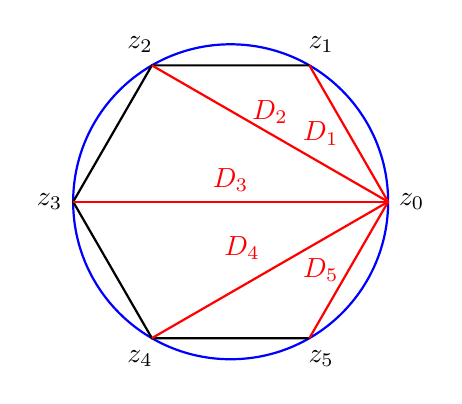
\begin{tikzpicture}[scale=2]
			\draw[thick, blue] (1, 0) arc (0:360:1cm);
			\draw[thick] (60:1cm) -- (120:1cm) -- (180:1cm) -- (240:1cm) -- (300:1cm);
			\foreach \x in {0, 1, 2, 3, 4, 5}
			\draw node at (60*\x:1.15cm) {\( z_{\x} \)};
			\draw[red, thick] (1, 0) -- node[midway, left] {\( D_1 \) } (60:1cm);
			\draw[red, thick] (1, 0) -- node[midway, above] {\( D_2 \) } (120:1cm);
			\draw[red, thick] (1, 0) -- node[midway, above] {\( D_3 \) } (180:1cm);
			\draw[red, thick] (1, 0) -- node[midway, above left] {\( D_4 \) } (240:1cm);
			\draw[red, thick] (1, 0) -- node[midway, left] {\( D_5 \) } (300:1cm);
		\end{tikzpicture}
	\end{center}
	For a general convex regular polygon described above, show that 
	\[
	\prod_{k = 1}^{N - 1}D_k = N
	\] 
\end{document}
